\documentclass[a4paper,11pt]{report}
\usepackage[T1]{fontenc}
\usepackage[utf8]{inputenc}
\usepackage{lmodern}
\usepackage{graphicx}

\title{\textbf{Sprawozdanie z laboratorium\\Sortowanie}}
\author{Adam Dąbrowski 184208}
\begin{document}
\maketitle
\section{Wprowadzenie}

Celem ćwiczenia było zapoznanie się z różnymi typami sortowania. Ja zaimplementowałem heapsort i quicksort. Oba te algorymtmy sortują w miejscu to znaczy nie wymagają żadnej dodatkowej struktury danych.  

\section{Realizacjia}

Program sprawdzam kolejno dla wielkości problemu 10, 100 ,1000,10 000, 100 000. Sortowanie przeprowadzam 50 razy, przy tej liczbie przy prawie każdym uruchomieniu dostaję podobne wyniki, a następnie liczę z tego średni czas. Dobrym punktem odniesienie przy analizie algorytmów sortowania jest podstawowe sortowanie bąbelkowe, ponieważ po kolei przestawia w tablicy wszystkie elementy- dlatego też swoją pracę zacząłem od napisanie tego tego typu sortowania. 
\section{HEAPSORT}

Złożoność obliczeniowa\\
Funkcja heapSort - $O(nlgn)$\\  
Funkcja buildMaxHeap - $O(n)$\\
Funkcja maxHeapify każde z n-1 wywołań - $O(lgn)$\\
\begin{tabular}{|rl|}
\hline
\multicolumn{2}{|c|}{HEAPSORT}\\
\hline
ilosc elementow & czas - nano sekundy\\
\hline
10&4099\\
100&41165\\
1000&301103\\
10000&3905768\\
100000&5820387\\
\hline
\end{tabular}
\\
\section{QUICKSORT}
Złożoność obliczeniowa w wypadku funkcji quicksort bardzo mocno zależy od danych wejśćiowych\\ 
W najgorszym wypadku-dane już posortowane $O(n^{2})$
Jednak zazwyczaj jest to $O(n lgn)$
  
\newpage
\begin{tabular}{|rl|}
\hline
\multicolumn{2}{|c|}{QUICKSORT- przypadek średni}\\
\hline
ilosc elementow & czas - nano sekundy\\
\hline
10&1725\\
100&26031\\
1000&144574\\
10000&1834571\\
100000&27507827\\
1000000&27507827\\
10000000&333791008\\
\hline
\end{tabular}
\\

\begin{figure}
  \begin{center}
    \includegraphics{wykresy/heapsort.eps}
    \caption{}
    \label{fig:}
  \end{center}
\end{figure}

\begin{tabular}{|rl|}
\hline
\multicolumn{2}{|c|}{QUICKSORT- przypadek najgorszy}\\
\hline
ilosc elementow & czas - nano sekundy\\
\hline
10&5035\\
100&334191\\
1000&7576229\\
10000&759267000\\
\hline
\end{tabular}
\\

\begin{figure}
  \begin{center}
    \includegraphics{wykresy/quicksort.eps}
    \caption{}
    \label{fig:}
  \end{center}
\end{figure}


\section{BUBBLESORT}

Złożoność obliczeniowa - $O(n^{2})$
  
\begin{tabular}{|rl|}
\hline
\multicolumn{2}{|c|}{BUBBLESORT}\\
\hline
ilosc elementow & czas - nano sekundy\\
\hline
10&3878\\
100&186381\\
1000&8346056\\
10000&769738534\\
\hline
\end{tabular}

\begin{figure}
  \begin{center}
    \includegraphics{wykresy/bubblesort.eps}
    \caption{}
    \label{fig:}
  \end{center}
\end{figure}


\section{Wnioski}
Quicksort w najgorszym wypadku podobnie jak bubblesort ma złożoność obliczeniową $O(n^{2})$, jednak dla przypadku średniego jest to $O(n lgn)$. Potwierdzają to otrzymane czasy realizacji gdzie quicksort(przypadek średni) byłem w stanie wywołać dla $n=10^{7}$ a bubblesort już tylko dla $n=10^{4}$. Dla przypadku najgorszego quickosrt otrzymane czasy realizacji były gorsze niż dla sortowania bąbelkowego. Czasy realizacji dla algorytmu heapsort zgodnie z założeniami teoretycznymi są bardzo zbliżone do tych quickort'a dla przypadku średniego.
\end{document}
